\documentclass[10pt]{beamer}
\usetheme{Malmoe}
\colorlet{beamer@blendedblue}{green!40!black}
\setbeamertemplate{navigation symbols}{}
\newcommand*\oldmacro{}%
\let\oldmacro\insertshorttitle%
\renewcommand*\insertshorttitle{%
\oldmacro\hfill%
\insertframenumber\,/\,\inserttotalframenumber}

\usepackage{xfrac}
\usepackage{caption}
\usepackage{hyperref}
\usepackage[makeroom]{cancel}
\usepackage{ amssymb }
\usepackage{appendixnumberbeamer}
%\usepackage{tikz-feynman}
\usepackage{graphicx}
\begin{document}
\title{Searching for Ultra Rare Processes Using the Large Hadron Collider}
\subtitle{$t \rightarrow q \gamma$}
\author[Barkeloo]{Jason Barkeloo}

\titlegraphic{
\includegraphics[width=4cm]{../ATLAS-Logo-Ref-RGB.png}\hspace*{2.75cm}~%
   
\includegraphics[width=4cm]{../uo_logo_green_on_white_2.jpg}
}

%\frame{\frametitle{}
%\begin{itemize}
%\item
%\end{itemize}
%}

\date{January 16, 2020}
\frame{\titlepage}
\frame{\frametitle{Overview}\tableofcontents[]}%hidesubsections]}
\section{The Large Hadron Collider}
%\frame{\frametitle{Table of Contents}\tableofcontents[currentsection,hideothersubsections]}
%%%%%%%%%%%%%%%%%%%%%%%%%%%%%%%%%%%%%%%%%%%%%%%%%%%%%%%%%
\subsection{LHC And ATLAS}
\subsection{Picking Through The Data}
\section{Search For Ultra Rare Decays}
\subsection{Machine Learning}


%%%%%%%%%%%%%%%%%%%%%%%%%%%%%%%%%%%%%%%%%%%%%%%%%%%%%%%%%%%%%%%%%%
\section{Outlook and Conclusions}

\frame{\frametitle{Outlook}
\begin{itemize}
\item Fake rates have been calculated and applied
\item Full systematics samples (slowly) running on the grid
\item Fitting machinery mostly in place now, should be ready once samples finish
\item Questions?
\end{itemize}
}



%%%%%%%%%%%%%%%%%%%%%%%%%%%%%%%%%%%%%%%%%%%%%%%%%%%%%%%%%%%%%%%%

\appendix
\section{Backup}
\frame{\frametitle{Backup}
}
\frame{\frametitle{FCNC Diagrams}
\centering
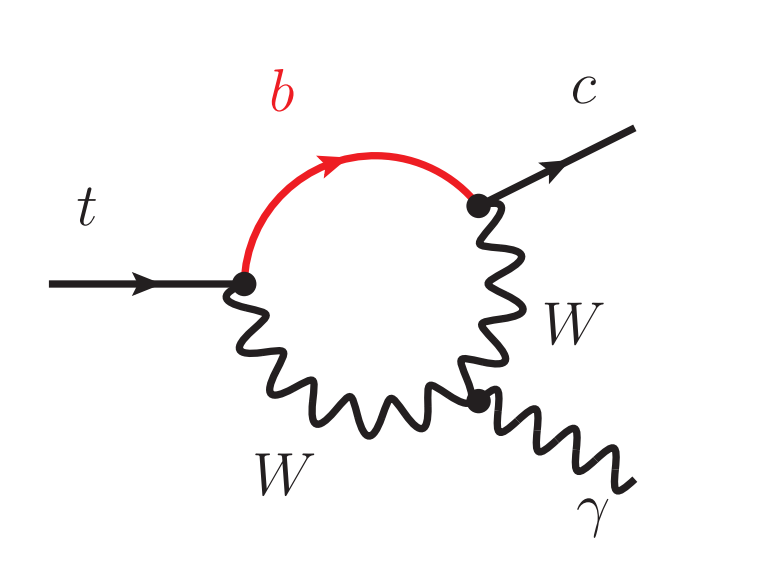
\includegraphics[width=.4\textwidth]{../../Thesis/ThesisImages/Theory/FCNCLoop.png}
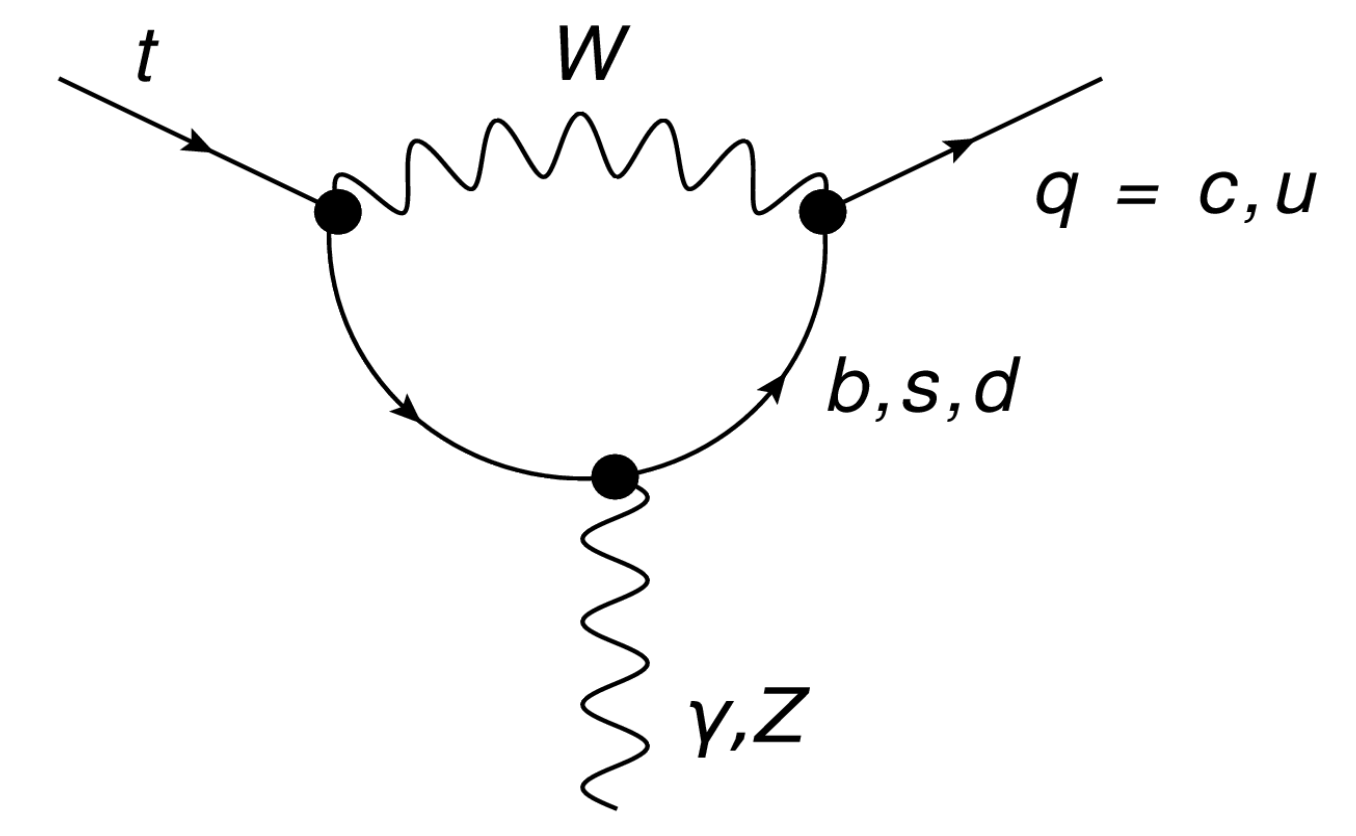
\includegraphics[width=.4\textwidth]{../../Thesis/ThesisImages/penguinFCNC.png}
}

\frame{\frametitle{No Photon Region SF Applied in Val Region}
\begin{columns}
\begin{column}{0.32\textwidth}
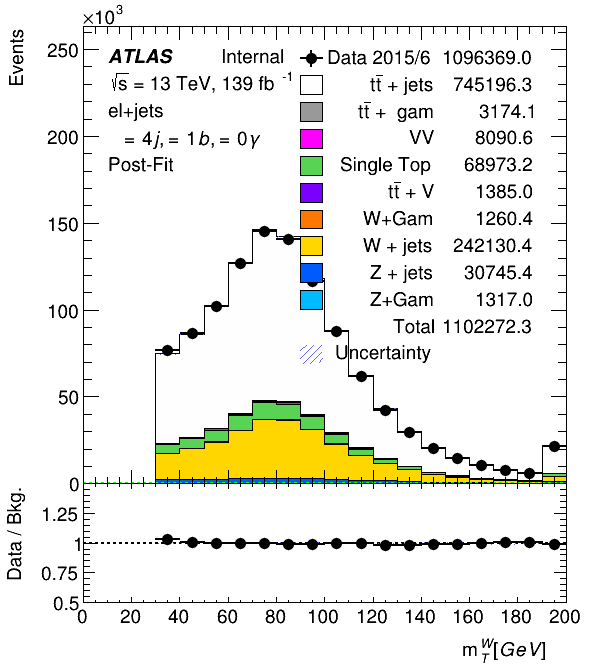
\includegraphics[width=.9\textwidth]{../../Thesis/ThesisImages/RegionPlots/AfterScaling/ControlRegions/HardCodedNormFactor/FCNC_All_ejets/Plots/VR3_MWT_postFit.png} \\
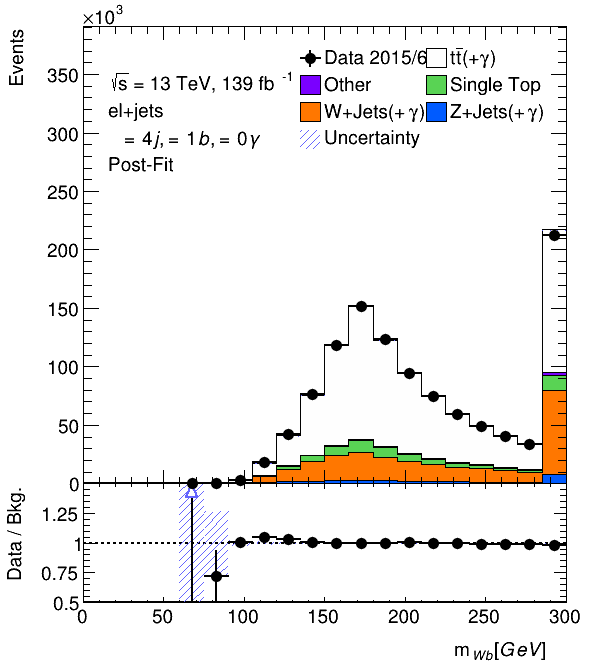
\includegraphics[width=.9\textwidth]{../../Thesis/ThesisImages/RegionPlots/AfterScaling/ControlRegions/HardCodedNormFactor/FCNC_All_ejets/Plots/VR3_SMtop_postFit.png} \\
\end{column}
\begin{column}{0.32\textwidth}
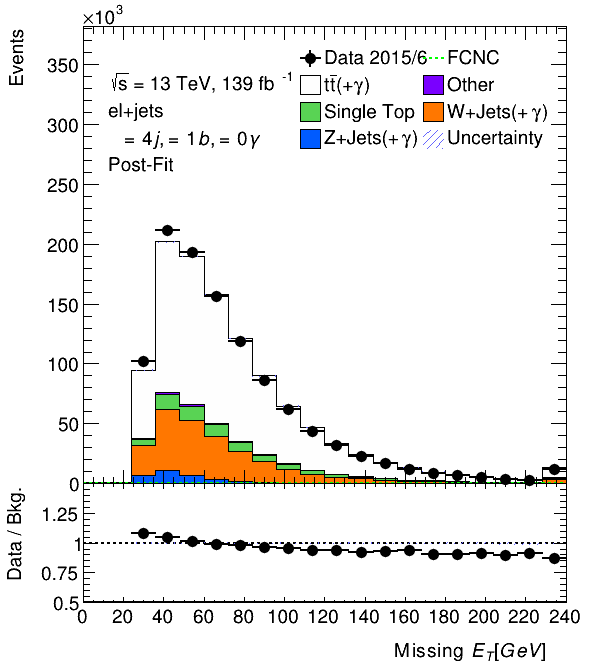
\includegraphics[width=.9\textwidth]{../../Thesis/ThesisImages/RegionPlots/AfterScaling/ControlRegions/HardCodedNormFactor/FCNC_All_ejets/Plots/VR3_met_postFit.png} \\
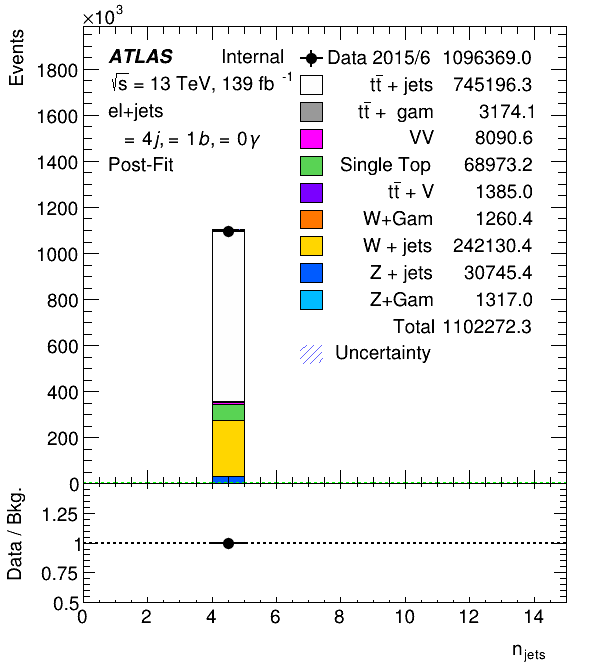
\includegraphics[width=.9\textwidth]{../../Thesis/ThesisImages/RegionPlots/AfterScaling/ControlRegions/HardCodedNormFactor/FCNC_All_ejets/Plots/VR3_njet_postFit.png}
\end{column}
\begin{column}{0.32\textwidth}
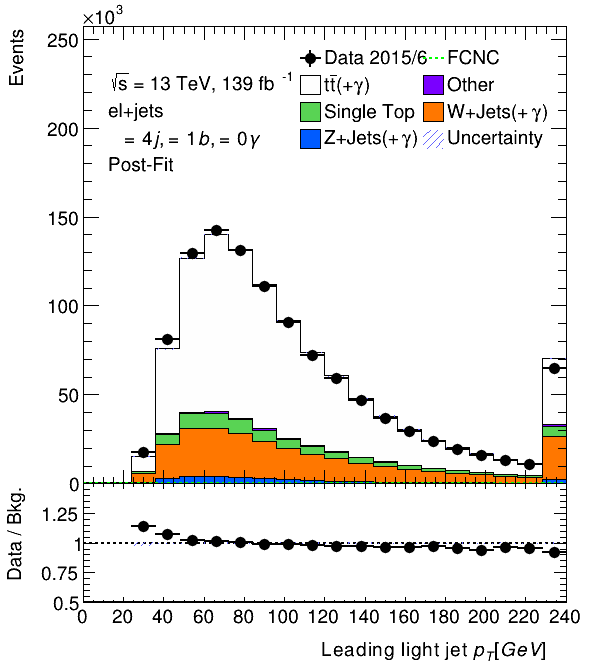
\includegraphics[width=.9\textwidth]{../../Thesis/ThesisImages/RegionPlots/AfterScaling/ControlRegions/HardCodedNormFactor/FCNC_All_ejets/Plots/VR3_jet0_pt_postFit.png} \\
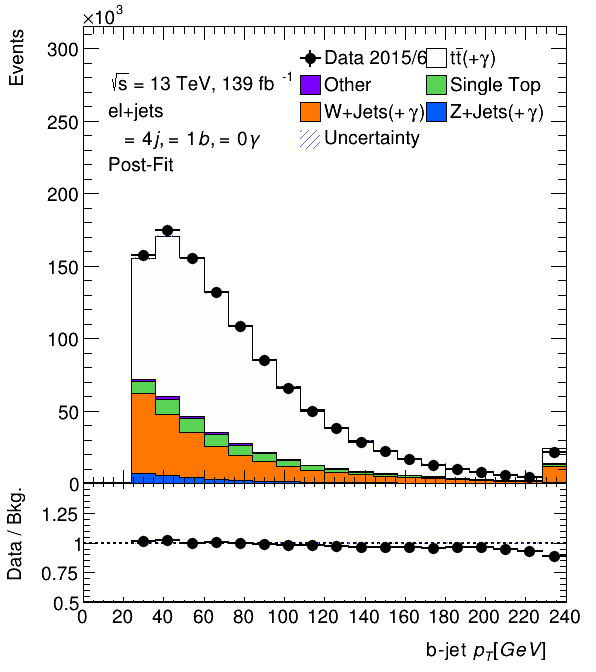
\includegraphics[width=.9\textwidth]{../../Thesis/ThesisImages/RegionPlots/AfterScaling/ControlRegions/HardCodedNormFactor/FCNC_All_ejets/Plots/VR3_bjet0_pt_postFit.png}
\end{column}
\end{columns}
}


%\frame{\frametitle{}
%}

%\frame{\frametitle{Neural Network Model Inputs}
%\centering
%\scalebox{0.8}{ $\text{Separation} = \sum_{i}^{bins} \frac {n_{s i}-n_{b i}}{n_{s i}+n_{b i}}$}
%\begin{columns}
%\begin{column}{0.48\textwidth}
%\centering
%mu+jets channel\\
%\scalebox{0.6}{\begin{tabular}{cc}
%Variable & Separation \\
%\hline
%photon0iso & 41.18 \\
%mqgam & 28.27 \\
%photon0pt & 24.07 \\
%mtSM & 11.60 \\
%mlgam & 7.56 \\
%deltaRjgam & 5.64 \\
%deltaRbl & 4.42 \\
%MWT & 3.34 \\
%ST & 3.30 \\
%nuchi2 & 3.12 \\
%jet0pt & 2.81 \\
%njets & 2.07 \\
%smchi2 & 1.89 \\
%wchi2 & 1.87 \\
%jet0e & 1.52 \\
%deltaRlgam & 1.17 \\
%leptone & 0.87 \\
%deltaRjb & 0.86 \\
%met & 0.68 \\
%bjet0pt & 0.52 \\
%leptoniso & 0.27 \\
%\end{tabular}
%}
%\end{column}
%\begin{column}{0.48\textwidth}
%\centering
%e+jets channel \\
%\scalebox{0.6}{\begin{tabular}{c c}
%Variable & Separation\\
%\hline
%photon0pt & 23.14 \\
%mqgam & 22.73 \\
%photon0iso & 18.70 \\
%mtSM & 11.02 \\
%mlgam & 9.53 \\
%deltaRbl & 5.00 \\
%deltaRjgam & 4.60 \\
%ST & 3.83 \\
%MWT & 3.16 \\
%jet0pt & 2.47 \\
%njets & 1.70 \\
%nuchi2 & 1.59 \\
%deltaRlgam & 1.40 \\
%wchi2 & 1.33 \\
%smchi2 & 1.09 \\
%deltaRjb & 0.88 \\
%leptone & 0.85 \\
%leptoniso & 0.56 \\
%bjet0pt & 0.50 \\
%met & 0.47 \\
%\end{tabular}
%}
%\end{column}
%\end{columns}
%}
%
%	\frame{\frametitle{Input Variables}
%	['photon0iso','photon0pt','mqgam','mlgam','mtSM','deltaRjgam','deltaRbl',\\
%	'MWT','ST','njets','wchi2','jet0pt','deltaRlgam','leptone','met','bjet0pt']
%	
%	
%	}

%\frame{\frametitle{Integrated Luminosity}
%\centering
%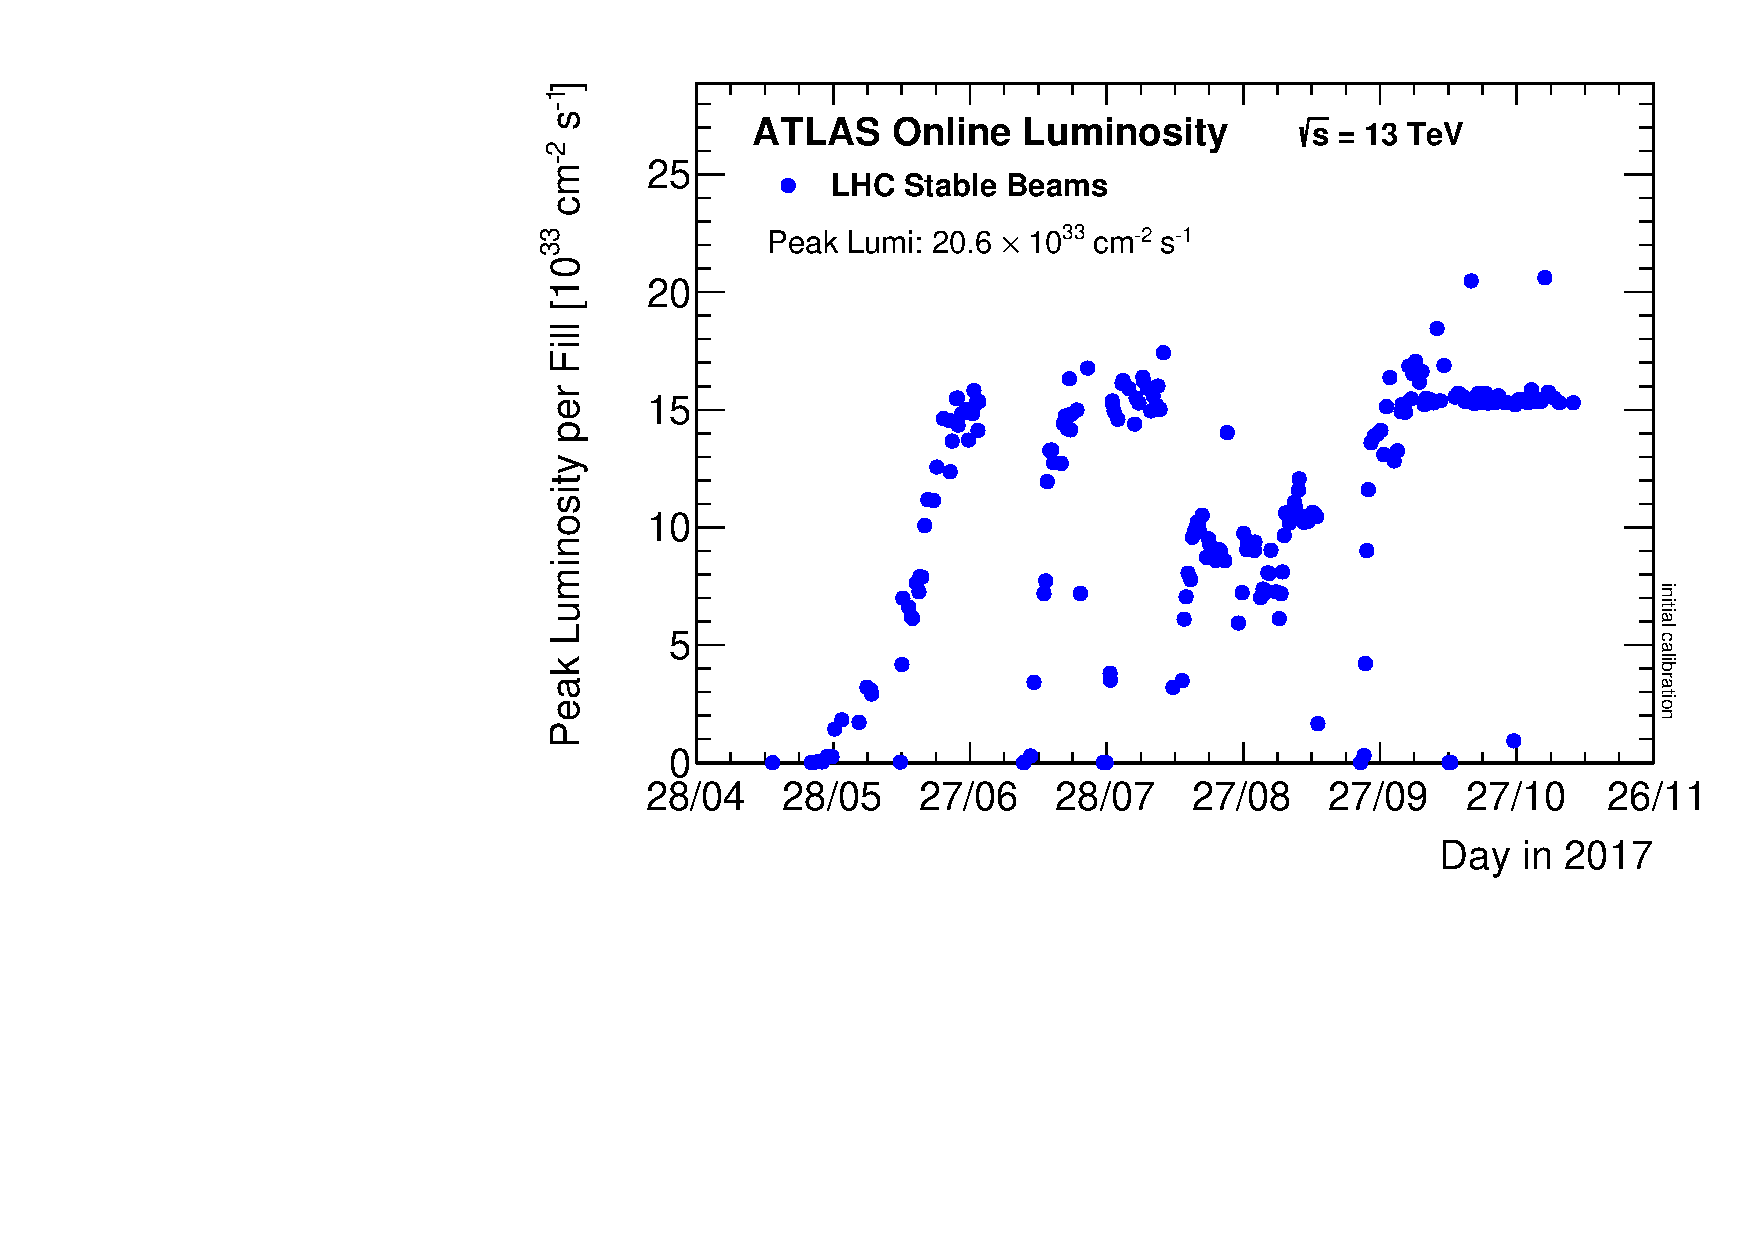
\includegraphics[width=1.\textwidth]{../../Thesis/ThesisImages/2017PeakLumiByFill.pdf}
%}
%\frame{\frametitle{A Couple BSM Diagrams}
%\centering
%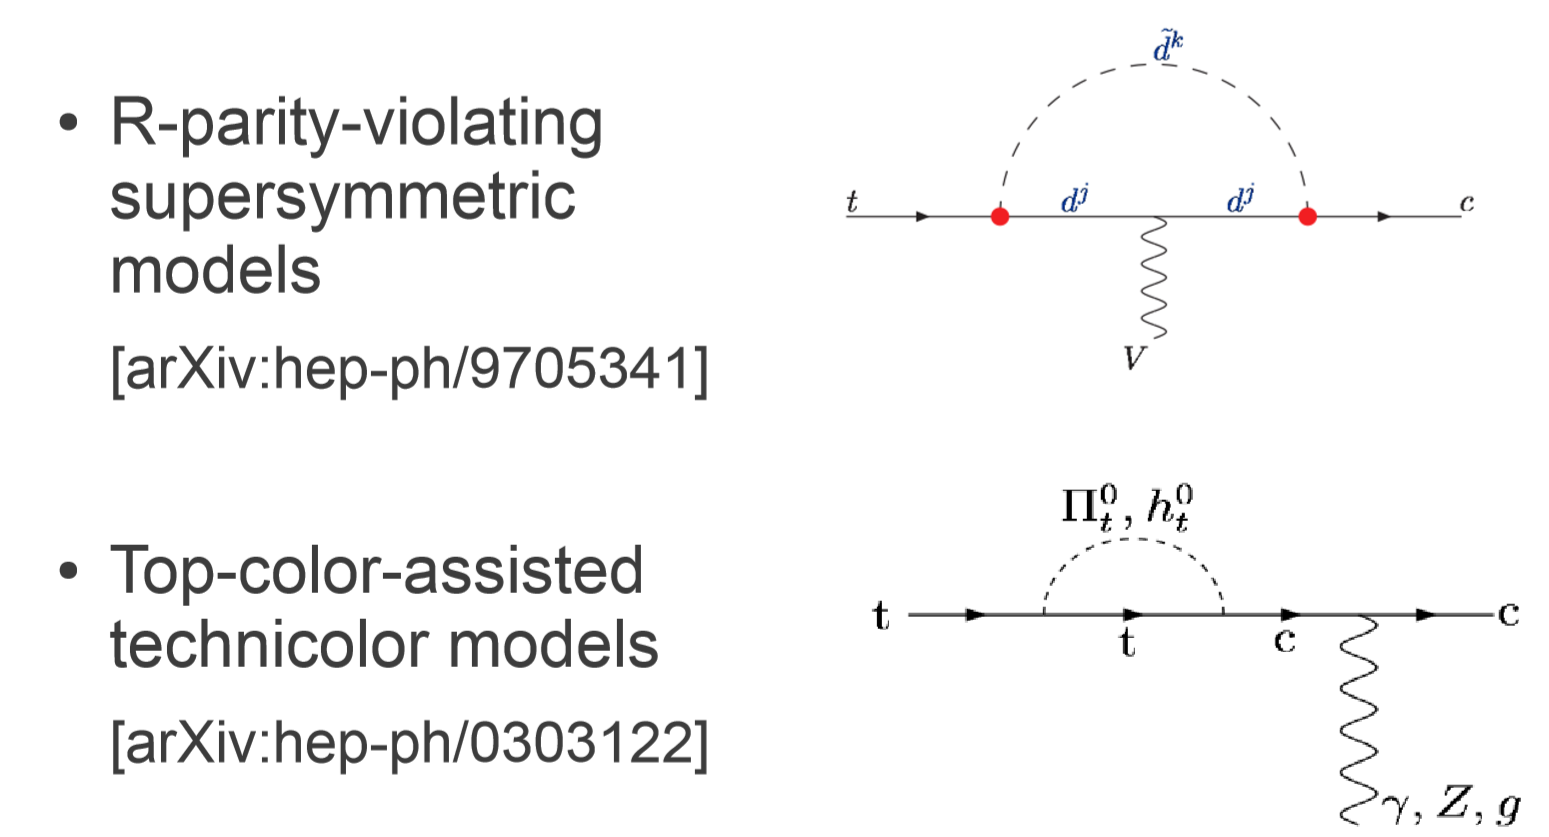
\includegraphics[width=1.\textwidth]{../../Thesis/ThesisImages/BSMDiagrams.png}
%}

\frame{\frametitle{Jets/AntiKT}

\[ d_{ij} = min(\frac{1}{p_{ti}^2},\frac{1}{p_{tj}^2}) \frac{\Delta_{ij}^2}{R^2}
\]
\[ d_{iB} = \frac{1}{p_{ti}^2}
\]
\[ \Delta_{ij}^2 = (\eta_i -\eta_j )^2 + (\phi_i - \phi_j )^2
\]
\begin{itemize}
\item Find minimum of entire set of $\{ d_{ij},d_{iB} \}$
\item If $d_{ij}$ is the minimum particles i,j are combined into one particle and removed from the list of particles
\item If $d_{iB}$ is the minimum i is labelled as a final jet and removed from the list of particles
\item Repeat until all particles are part of a jet with distance between jet axes $\Delta_{ij}$ is greater than R
\end{itemize}
}

%\frame{\frametitle{B-tagging}
%\centering
%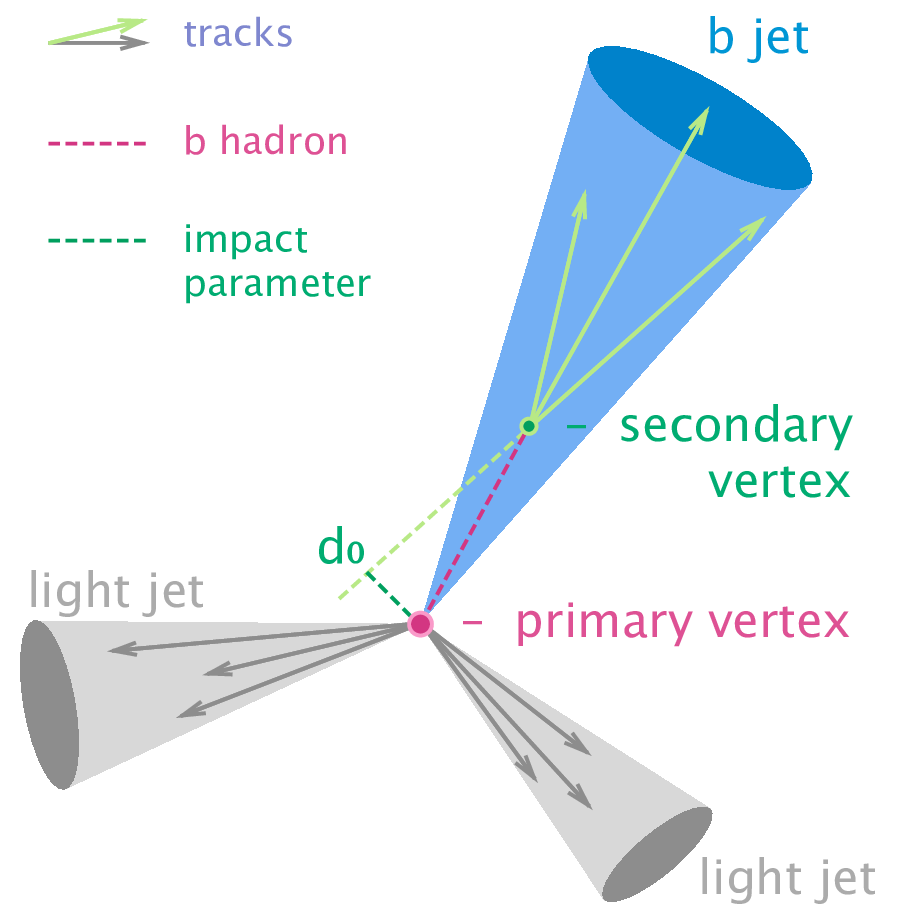
\includegraphics[height=.8\textheight]{../../Thesis/ThesisImages/SimulationNN/B-tagging_diagram.png}
%}

\frame{\frametitle{}
\[ \mathcal{L}^{eff}_{tq\gamma} = - e \bar{c} \frac{i \sigma^{\mu\nu}q_{\nu}}{m_t}(\lambda^{L}_{ct}P_L + \lambda^{R}_{ct}P_{R}) t A_{\mu} +H.c.
\]
}

\end{document}

%36.070


%%% Neural Net Ref: http://cs231n.github.io/neural-networks-1/

% npart0=['photon0_iso','photon0_pt','m_qgam','m_lgam','m_tSM','deltaRjgam','deltaRbl','MWT','S_T','nbjets','njets','w_chi2','jet0_pt','nu_chi2','sm_chi2','deltaRlgam','lepton_e','met','lepton_iso','bjet0_pt']
%all vars

%npart = ['photon0_iso','photon0_pt','m_qgam','m_lgam','m_tSM','deltaRjgam','deltaRbl','MWT','S_T','njets','nbjets','w_chi2','jet0_pt','deltaRlgam','lepton_e','met','bjet0_pt']
%usual npart1

%npart1=['photon0_iso','photon0_pt','deltaRjgam','deltaRbl','MWT','S_T','njets','w_chi2','jet0_pt','deltaRlgam','lepton_e','met','bjet0_pt']
%minimal